\documentclass[a4paper,12pt, fleqn]{article}
\usepackage{amsmath}
\usepackage[hmargin=1in,vmargin=1in]{geometry}
\usepackage{enumerate}
\usepackage{graphicx,float}
\usepackage{hyperref}
\pagestyle{empty}
\linespread{1.5}
\begin{document}
\begin{center}
\Large
\textbf{AMATH 481/581 - Autumn 2022}
\textbf{Homework \#3}
\textbf{Sathvik Chinta}
\normalsize
\end{center}
\begin{enumerate}
    \item 
        \textbf{Presentation Skills:} To earn mastery in discussing problems
        from a physical perspective, discuss what $c(x,t)$ means and how it
        impacts the solution. Discuss the difference in the solution from
        $c(x,t) = -0.5$ and $c(x,t) = -\left(1 + 2\sin(5t) - H(x-4)\right)$.
        What does this non-constant speed correspond to? How does it affect the
        solution? Does this agree with your intuition? You should create and
        use the figures from (b) and (c) to backup your arguments. 
        (Hint: The velocity field has two components: one temporal (time) and
        one spatial. How does each component factor in?)\\

        \textbf{Introduction}\\
        In this problem, we solved the advection flow equation and investigated 
        the impact of a velocity field on the physical model. We analyze two
        velocity fields, $c(x,t) = -0.5$ and $c(x,t) = -\left(1 + 2\sin(5t) - H(x-4)\right)$ 
        which we model as a constant and non-constant velocity field respectively. In 
        the non-constant velocity field, we add a time ($t$) dependence as well as a 
        spatial ($x$) dependence. The time dependence can be described by the governing 
        equation $2\sin(5t)$, thus we expect the velocity field to be sinusoidal in
        the temporal domain. The spatial dependence is described by the Heaviside
        function $H(x-4)$, which is 1 for $x > 4$ and 0 for $x \leq 4$. Thus, we expect
        the velocity field to be 1 for $x > 4$ and 0 for $x \leq 4$.\\

        The Heaviside function can be described as follows:\\

        \begin{equation}
            H(x) = \begin{cases}
                1 & x > 0 \\
                0 & x \leq 0
            \end{cases}
        \end{equation}\\


        \textbf{Results and Analysis}

        Looking at $c(x, t)$ in two different scenarios, we can see clear differences. 
        In the first instance, there is a constant speed of $c(x,t) = -0.5$. The graph for
        the solution with this constant speed is shown below.\\

        \begin{figure}[H]
            \centering
            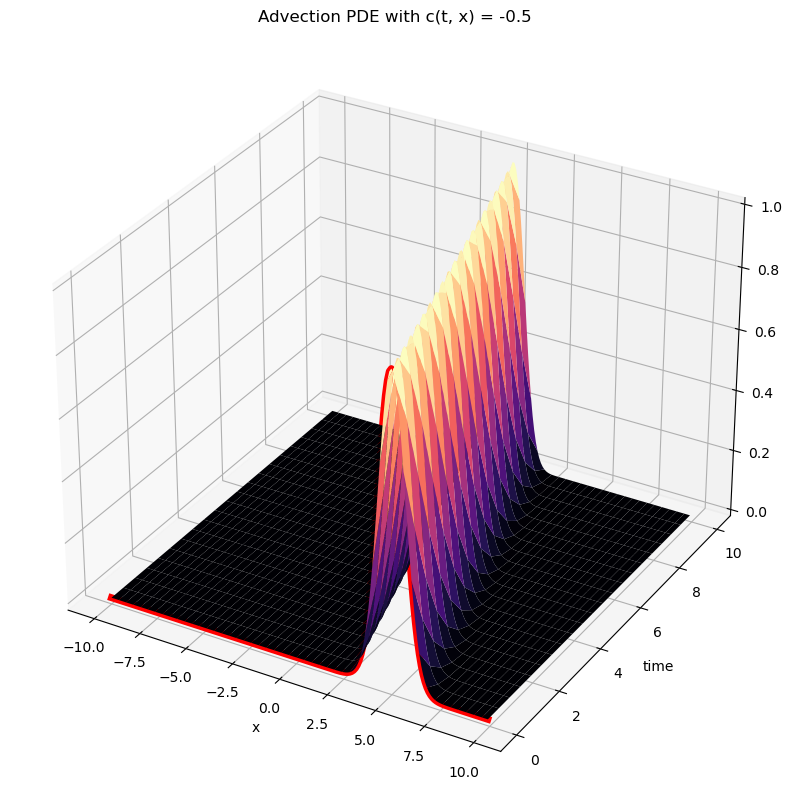
\includegraphics[width=0.45\textwidth]{/workspaces/AMATH-481/constant.png}
            \caption{Solution with constant speed $c(x,t) = -0.5$}
            \label{fig:hw3-1a}
        \end{figure}

        We can see that the peaks of the waves are the same height, and as time increases, the
        waves move to the left in the x-axis. 

        In the second instance, we have a non-constant speed of 
        $c(x,t) = -\left(1 + 2\sin(5t) - H(x-4)\right)$. The graph for the solution with this
        non-constant speed is shown below.\\

        \begin{figure}[H]
            \centering
            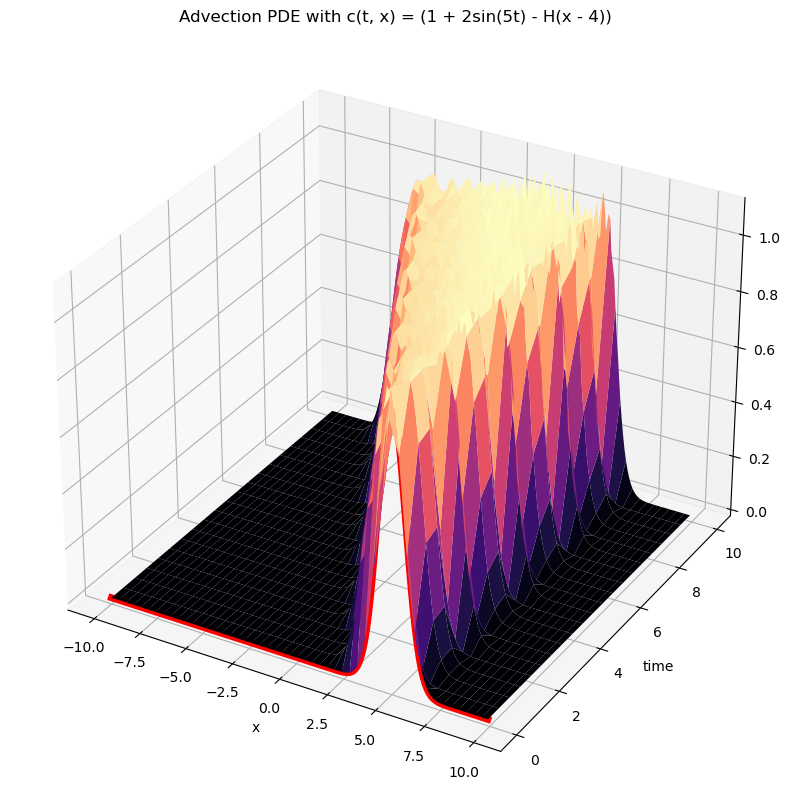
\includegraphics[width=0.45\textwidth]{/workspaces/AMATH-481/changing.png}
            \caption{Solution with non-constant speed $c(x,t) = -\left(1 + 2\sin(5t) - H(x-4)\right)$}
            \label{fig:hw3-1b}
        \end{figure}

        Now, we can see a clear change in the solution. There is a spatial dependency, as the 
        peaks in our waves are not at the same height at all points in the x-axis. Furthermore, 
        there is a temporal dependency as we see the waves spread out the further out in time that 
        we go. 

        This agrees with our intuition. In the first instance, we have no time dependency. As such, 
        we saw the waves stay contant in shape and height as we moved through time. When we added the
        temporal and spatial dependencies, we saw the waves change shape and height as we moved through
        both time and space. We no longer have a uniform shape, as we see a various arrray of heights. 
        Furthermore, we see the waves spread out and create a "wedge" shape in our graph as well. 

        We can view this model similarly to that of a wave pool. The waves bouncing back from the edges
        of the wave pool create irregularities in our wave, causing a spatial distortion. As the amount of waves 
        bouncing back increases, the waves are more distorted. The amount of waves being bounced back is directly 
        related to the time since the wave created, thus we see a temporal dependency as well. 

        \textbf{Conclusion and Future Work}

        In this problem, we analyzed the impact of a constant and non-constant velocity field on the solution to the
        advection flow equation. We saw that the non-constant velocity field created a spatial and temporal dependency
        in our solution, and saw how it effected the shape of our waves. Adding a sinusoidal time dependence along with a 
        heaviside spatial dependence creates distortion in our waves, which is similar to the distortion we see in a wave pool.

        For future work, we can investigate velocity fields that have only a spatial or temporal dependence, and compare 
        the results to what we have investigated in this problem. We can also investigate the use of more complex
        veolocity fields that are governed by their own ordinary differential equations, creating more chaos in 
        our model in order to investigate the results. 

    \item    
        \textbf{Presentation Skills:} To earn mastery in \textit{discussing problems from a
        mathematical perspective}, compute how long it takes to solve
        this PDE using Gaussian Elimination and LU decomposition. Do
        this for the specified grid size here and with 128 points in
        the $x$ and $y$ directions. Discuss the times that you find.
        Does it surprise you is it as you expect? Explain why it is as
        you expect or not. 

        \textbf{Introduction}\\
        In this problem, we are asked to compute the time it takes to solve the coupled vorticity
        and stream function equations. We solve by first discretizing the equations and then
        performing matrix operations to solve for our final solution. During this process, 
        we inevitably have to solve a linear system of equations. We can solve this system
        using Gaussian Elimination or LU decomposition. The time it takes to solve the system, 
        and ultimately the PDE, is thus dependent on how long these two methods take. We 
        analyze the time it takes to solve the system using both methods.

        
        \textbf{Results and Analysis}
        % Create a table with the times for each method and grid size

        \begin{table}[H]
            \centering
            \begin{tabular}{|c|c|c|}
                \hline
                \textbf{Method} & \textbf{Grid Size} & \textbf{Time}\\
                \hline
                Gaussian Elimination & 64 & 2.393669 \\
                Gaussian Elimination & 128 & 14.261790 \\
                LU Decomposition & 64 &  0.108140\\
                LU Decomposition & 128 & 0.230667 \\
                \hline
            \end{tabular}
            \caption{Times for solving the PDE using Gaussian Elimination and LU Decomposition}
            \label{tab:hw3-1c}
        \end{table}

        We can see that in both cases, the time taken to solve using LU is significantly 
        less than the time taken to solve using Gaussian Elimination. When we solved using 
        LU decomposition, we moved the $A$ matrix into a lower triangular matrix and an upper
        triangular matrix. This calculation was done \textbf{outisde of our loop}, meaning
        the operation was only performed once. Then, we could  use the lower and upper triangular
        matrices to solve for our $\psi$ vector within the loop. When comparing to the Gaussian, 
        we had to perform Guassian elimination on our $A$ matrix every time we went through the 
        loop, and then immediately solve for $\psi$ in addition to that. Thus, it stands to reason 
        that just by the sheer amount of operations performed within the loop every time, 
        the LU decomposition method would be faster.

        One interesting point to note, however, is how the time taken to solve the PDE scales
        with size. While the LU Decomposition time scaled linearly (~2 times as long for a 
        grid size that was twice as big), the Gaussian Elimination time was almost 7 times as 
        slow! This is because the Gaussian Elimination method is an $O(n^3)$ algorithm, while the
        LU Decomposition method is an $O(n^2)$ algorithm (solving for the LU decomposition of the 
        $A$ matrix is $O(n^3)$, but that operation is only performed once). So, the larger
        the grid size, the greater the difference in the time taken to solve the PDE for these 
        two methods. 

        \textbf{Conclusion and Future Work}

        In this problem, we analyzed the time it takes to solve the coupled vorticity and stream
        function equations using Gaussian Elimination and LU Decomposition. We saw that the LU
        Decomposition method was significantly faster than the Gaussian Elimination method, and
        that the time taken to solve the PDE scaled linearly with the grid size.

        For future work, we can investigate the time it takes to solve the PDE using other methods
        such as Jacobi or Gauss-Seidel.
        
        To compare the differences in time complexity, we can plot a graph of the time taken to
        solve the PDE for each method as a function of the grid size. Furthermore, we can examine the
        results if we were to repeat the LU Decomposition every time as we went through the loop. 
        From our analysis thus far, we would imagine the two methods to have similar times in 
        this scenario. 
\end{enumerate}
    
\end{document}